\section{Desarrollo}

En esta sección damos un detalle de las estructruas que utilizamos para mantener la contención y sincronización entre los diferentes hilos del proceso. Luego, explicamos a alto nivel el pseudocódigo correspondiente a nuestro algoritmo.

\subsection{Estructuras}

\begin{figure}[h]
    \centering
    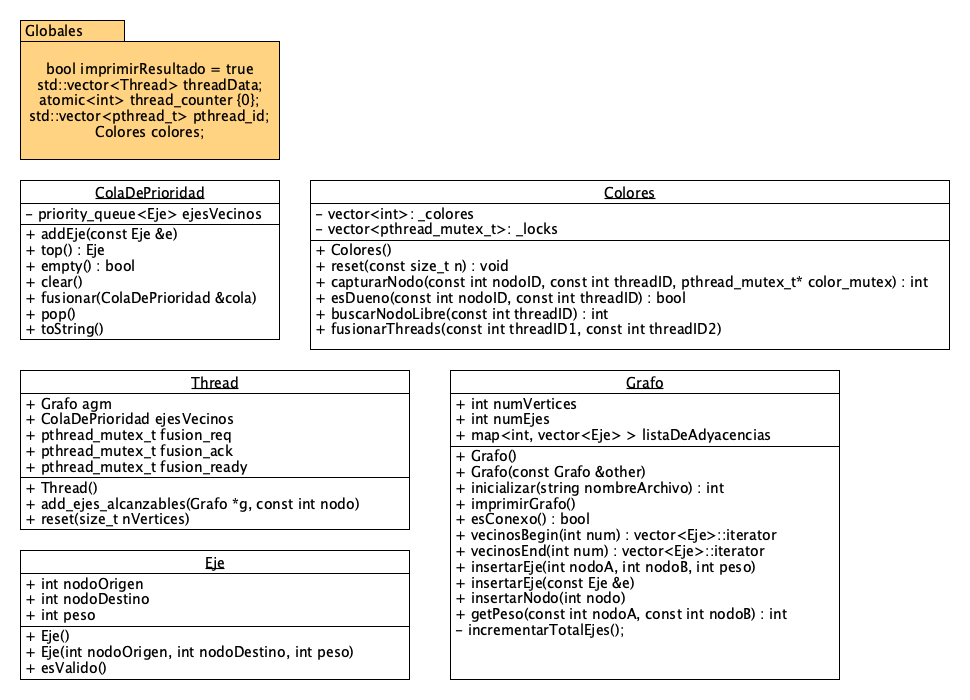
\includegraphics[width=1\textwidth]{imagenes/tp1.png} \\%
    \caption{Clases y estructuras}
    \label{fig:uml}
\end{figure}

\subsubsection{Variables globales}

En la memoria compartida por cada proceso se encuentra la información correspondiente a cada thread en \textbf{threadData}, el \textit{ownership} de cada nodo en \textbf{colores}, un contador atómico para identificar los threads durante su inicialización, \textbf{thread_counter} y finalmente un vector de \textit{pthread_t} para coordinar la creación de los threads y para esperar a que los mismos terminen: \textbf{pthread_id}.

Estos objetos se encuentran en: \textmd{/src/globales.h}

\subsubsection{Grafos y Ejes}

Se utilizaron las estructuras facilitadas por la cátedra con leves modificaciones. En el caso de los grafos se agregó un constructor por copia y se sobrecargó el método de \textbf{insertarEje}, también incluyeron: \textbf{insertarNodo} y \textbf{getPeso} para facilitar algunas operaciones.

En el caso de los ejes, se agregó información correspondiente al nodo de origen y un constructor con distintos parámetros.

Ver \textmd{/src/grafo.h}

\newpage

\subsubsection{Thread}

\begin{verbatim}
    struct Thread{
        Grafo agm;
        ColaDePrioridad ejesVecinos;
        pthread_mutex_t fusion_req;
        pthread_mutex_t fusion_ack;
        pthread_mutex_t fusion_ready;
    };
\end{verbatim}

Trabajamos con esta estructura para resguardar la información de cada thread. La misma consiste de un grafo que será el AGM parcial del thread, una cola de prioridad que contiene a los ejes cuyo nodo destino es alcanzable desde el AGM y tres mutex para administrar las fusiones. Tendremos un vector global que contendrá uno de estos structs por cada thread, el nombre del mismo es threadData.

Ver \textmd{/src/thread.h}

\subsubsection{Cola De Prioridad}

Cada thread tiene una cola de prioridad, \textbf{ejesVecinos}, que mantiene ordenados crecientemente los ejes actualmente alcanzables según su peso. A la hora de buscar el próximo nodo a capturar, siempre se eligirá el primer elemento de la cola. Luego de capturar un nodo, sus ejes son agregados a la misma y el proceso se repite.

Ver \textmd{/src/cola_proridad.h}

\subsubsection{Colores}

\begin{verbatim}
    class Colores {
        vector<int> _colores;
        vector<pthread_mutex_t> _locks;
    };
\end{verbatim}

Para controlar que la pertenencia de los nodos del grafo utilizamos esta estructura que contiene un vector con el color de cada uno, los cuales no son otra cosa que los ID de cada thread. Para evitar race conditions y asegurar contención, cada nodo tiene además un mutex asociado el cual nos permite tener acceso exclusivo al mismo. Vamos a distinguir además a los nodos libres con un -1.  Las operaciones principales de la clase son \textbf{esDueño} que nos permite conocer al thread que posee a ese nodo y \textbf{capturarNodo} cuyo objetivo es convertir a un thread en dueño de un nodo. En caso de que esto ultimo no sea posible, porque ya pertenece a otro thread, se procederá a solicitar una fusión. Cuando esta se produzca los nodos del thread de mayor id cambiaran de dueño y pasaran a ser del de menor id.

Ver \textmd{/src/colores.h}

\subsubsection{Fusión}

Como mencionamos anteriormente, cada thread cuenta con tres mutex para administrar tanto la solicitud como la habilitación de fusiones. En cada ciclo los threads van a chequear si tienen fusiones entrantes haciendo trylock de su mutex fusion\_req. Mientras no puedan tomarlo implica que otro thread está esperando para fusionarse. Si lo pueden tomar, se hace un unlock de su fusion\_ack despertando al thread solicitante y un lock de fusion\_ready, este último es para esperar a que el otro thread solicitante termine de realizar la fusión.

Una vez que ya no tiene pendientes procede a buscar el próximo nodo e intentar capturarlo. En caso de que pertenezca a otro thread solicita una fusión de la siguiente forma: primero chequea que no tenga funciones entrantes haciendo un trylock de su fusion\_req. Esto lo hacemos para evitar un posible deadlock. Luego, lo mismo pero con el fusion\_req del thread dueño del nodo que quiere capturar. Si puede conseguirlo hace lock del fusion\_ack del otro thread quedando así en espera hasta que el mismo esté preparado para realizar la fusión. Una vez que la misma se produce se verifica que el dueño siga siendo el mismo ya que podría haber ocurrido una fusión y por lo tanto haber cambiado. Si se mantuvo se debe chequear cuál es el de menor id, el cual será quien "sobreviva". El otro será reiniciado y comenzará de nuevo con todo el proceso. El sobreviviente tendrá ahora la unión de ambos AGMs y ambas colas de prioridad.

Por ultimo, ambos fusion\_req serán desbloqueados, así como el fusion\_ready del perdedor. Es importante remarcar que el thread reiniciado mantiene el estado de sus mutex ya que, si no, podría ocurrir que algún thread quede esperando fusionarse con él. Si no hubiera sido posible conseguir alguno de los fusion\_req o el dueño del nodo hubiera cambiado el thread habría vuelto al principio de este ciclo.

Ver \textmd{/src/fusiones.h} y \textbf{mstParaleloThread} en \textmd{/src/tp1_grafo.cpp}

\subsection{Algoritmo}

\begin{algorithm}
    \begin{algorithmic}
        \caption{mstParaleloThread}
        \Function{mstParalelothread}{grafo}
            \STATE $my\_id \gets thread\_counter++ $
            \STATE $eje\_actual$
            \STATE $my\_data \gets threadData[my\_id]$
            \WHILE{$true$}
                \STATE $thread\_attend\_fusion\_requests(my\_id)$
                \STATE $my\_data.fusion\_req.unlock()$
                \STATE $status \gets buscarNodo(my\_id,ejeActual)$
                \IF{($status = noHayNodosDisponibles$)}
                    \STATE $thread\_attend\_fusion\_requests(my\_id)$
                \ENDIF
                \IF{($status = agmCompleto$)}
                    \STATE $break$
                \ENDIF
                \STATE $owner\_id \gets colores.capturarNodo(ejeActual.nodoDestino,my$\textunderscore$id)$
                \IF{($my\_id = owner\_id$)}
                    \STATE $my\_data.insertarEje(ejeActual)$
                    \STATE $my\_data.agregarEjesVecinos(g,ejeActual.nodoDestino)$
                \ELSE 
                    \STATE $owner\_data \gets threadData[owner\_id]$
                    \IF{($my\_data.fusion\_req.trylock() \neq 0 )$}
                        \STATE $continue$
                    \ENDIF
                    \IF{($owner\_data.fusion\_req.trylock() \neq 0$)}
                        \STATE $my\_data.fusion\_req.unlock()$
                        \STATE $continue$
                    \ENDIF
                    \STATE $owner\_data.fusion\_ack.lock()$
                    \IF{($colores.esDueno(ejeActual,owner\_id)$)}
                        \STATE $my\_data.agm.insertarEje(ejeActual)$
                        \IF{($my\_id < owner\_id $)}
                            \STATE $fuse(my\_id,owner\_id)$
                        \ELSE
                            \STATE $fuse(owner\_id,my\_id)$
                        \ENDIF
                    \ENDIF
                \ENDIF
                \STATE $owner\_id.fusion\_req.unlock()$
                \STATE $my\_id.fusion\_req.unlock()$
                \STATE $owner\_id.fusion\_ready.unlock()$
            \ENDWHILE
    \end{algorithmic}
\end{algorithm}

\newpage

Aclaraciones:
\begin{itemize}
    \item No realizamos copias del threadData en la implementación. Esto es solamente para clarificar el pseudocódigo.
    \item $thread\_attend\_fusion\_requests$ realiza el chequeo de las funciones entrantes como se explica en la sección 2.1.3.
    \item La idea de buscarNodo es que encuentre el próximo nodo a agregar al agm del thread. Si aun no tiene ninguno toma el primero libre que encuentre. Sino al nodo alcanzable cuyo eje es de peso mínimo. Además de devolver un status retorna el eje en ejeActual.
\end{itemize}
